\chapter{RIC Near-Real-Time}

یکی از اجزای اصلی
\lr{O-RAN}،
\lr{Near-Real-Time RIC} 
است که وظیفه‌ی کنترل هوشمندانه‌ی ناحیه دسترسی رادیویی با تاخیر نسبتا کم و به صورت نزدیک به بلادرنگ را برعهده دارد.

این قسمت همان‌طور که در 
\ref{fig:nrt-ric0}
هم مشاهده می‌شود، خود از قسمت‌های زیادی تشکیل شده که در ادامه هر کدام از آن‌ها معرفی خواهند شد.

\begin{figure}[H]
	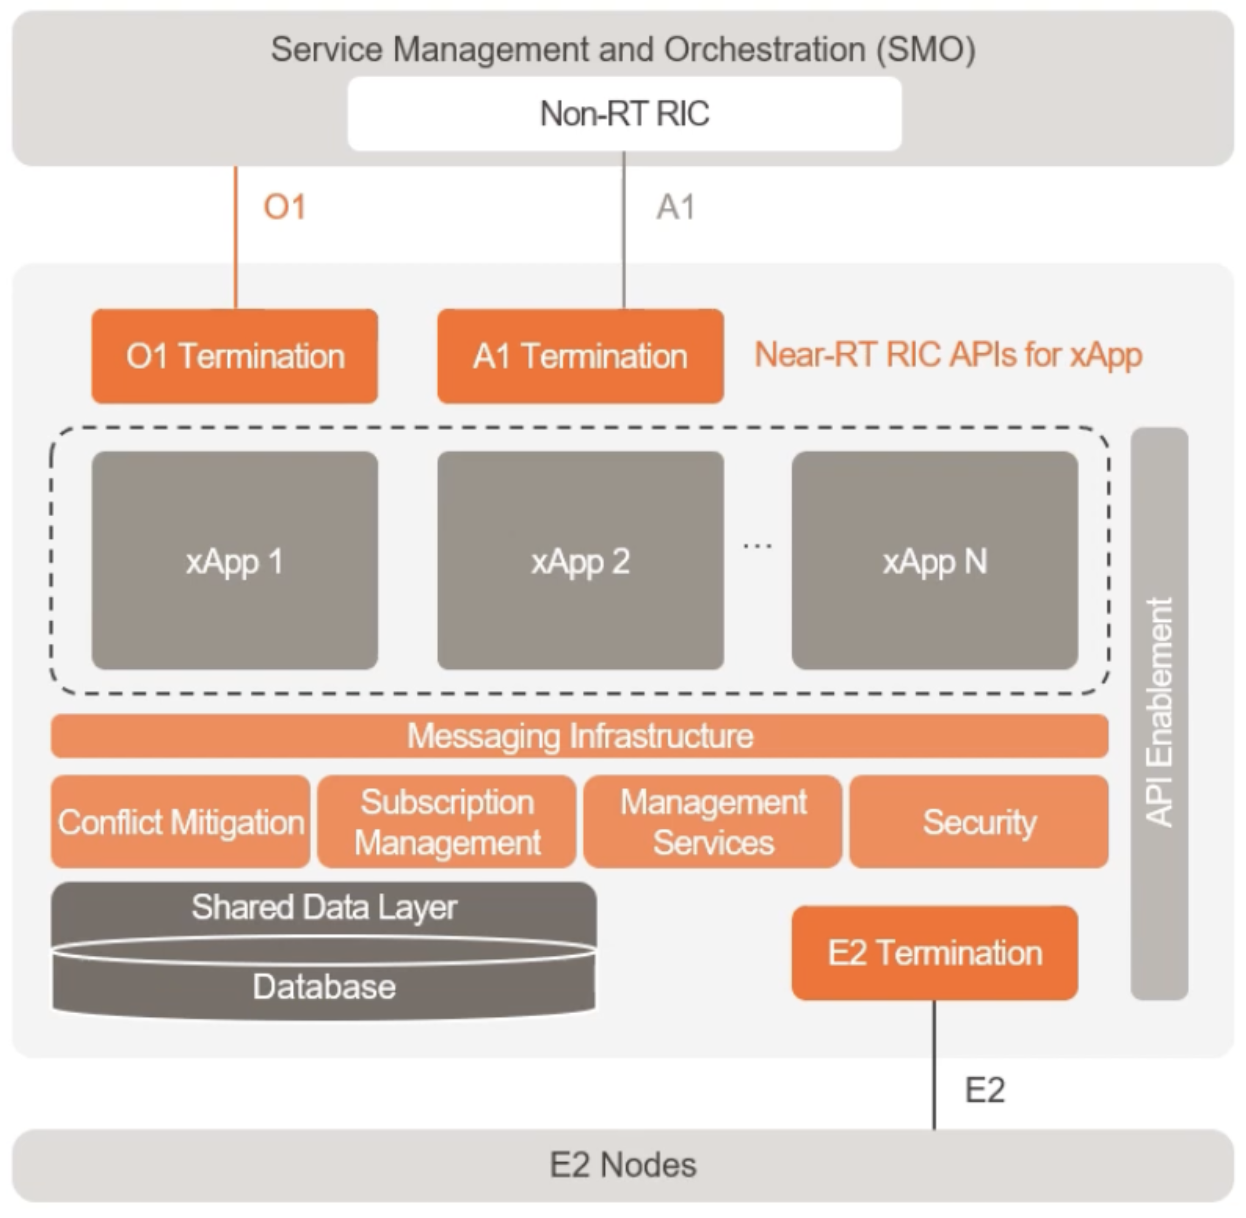
\includegraphics[width=0.85\columnwidth]{Picture/nrt-ric0.png}
	\centering
	\caption{اجزای مختلف موجود در
	\lr{Near-Real-Time RIC}}
	\label{fig:nrt-ric0}
\end{figure}

\section{\lr{xApp}}
اصلی‌ترین مفهوم در 
\lr{Near-Real-Time RIC} 
همین مفهوم یعنی 
\lr{xApp} 
است. 
\lr{xApp}ها
یک سری برنامه‌ی کوچک اند که از طریق آن‌ها تصمیم‌های کنترلی به کمک داده‌هایی که به عنوان ورودی به آن‌ها داده می‌شود، گرفته می‌شود. این تصمیم‌ها از طریق واسط
\lr{E2}
که در فصل‌های بعدی معرفی می‌شود، به دست 
\lr{DU} یا
\lr{CU}
می‌رسد تا اجرایی شوند.

\begin{note}
نحوه‌ی عملیاتی کردن این برنامه‌ها در ساختار
\lr{O-RAN}
عموما به صورت 
\lr{image}های
\lr{docker}ی
است و یک فایل پیکره‌بندی که مشخصات بالا آمدن هر کدام از این برنامه‌ها را دقیق‌تر مشخص می‌کند.
\end{note}


\section{\lr{Messaging Infrastructure}}
این بخش یک زیرساخت پیام‌رسانی است که پیغام‌های مختلف بین اجزای مختلف موجود در
\lr{Near-Real-Time RIC} 
از طریق آن رد و بدل می‌شود. 

\section{\lr{Conflict Mitigation}}
این بخش وظیفه دارد تا از بروز اشکالاتی که به خاطر تداخل پیکره‌بندی‌های مختلفی که 
\lr{xApp}ها
به وجود می‌آورند جلوگیری کند یا اینکه با مکانیزم‌های خود، آن‌ها را تشخیص دهد و سپس آن‌ها را اصلاح کند. به صورت ساده‌تر این قسمت از دست‌کاری موارد یکسان توسط برنامه‌های مختلف که ممکن است باعث خرابی عملکردی شود، جلوگیری می‌کند.

\section{\lr{Subscription Manager}}
این بخش بررسی و مدیریت اینکه
\lr{xApp}های
مختلف به 
\lr{E2}
نودهایی (همان 
\lr{DU}
و
\lr{CU})
که می‌خواهد اطلاعات از آن‌ها دریافت کند، درخواستشان را ارسال کنند را برعهده دارد. به عنوان مثال اگر چندین برنامه نیازمند به یک مرجع داده‌ی یکسان داشته باشند، این بخش این درخواست‌ها را تجمیع می‌کند تا مدیریت و کنترل‌ آن‌ها ساده‌تر باشد.

\section{\lr{Management Services}}
این بخش وظیفه‌ی مدیریت خود
\lr{xApp}ها،
ساختار عیب‌یابی و عملیاتی کردن آن‌ها و به صورت کلی موارد مرتبط با خود 
\lr{xApp}ها
را بر عهده دارد.

\section{\lr{Security}}
 با توجه به اینکه اطلاعات موجود در ناحیه‌ی دسترسی رادیویی، اطلاعات محرمانه‌ای در مورد کاربران را شامل می‌شود، این قسمت وظیفه‌اش حفظ امنیت این داده‌ها است. البته هنوز در پیاده‌سازی‌هایی که انجام شده به سراغ این موضوع به صورت جدی نرفته‌اند و در دست پیشرفت است.
 
\section{\lr{Database}}
 این قسمت هم، همان‌طور که نامش پیداست،‌ پایگاه داده‌ای است که اطلاعات مختلف کاربران را نگه‌داری می‌کند تا 
 \lr{xApp}های
 مختلف در صورت نیاز بتوانند از آن‌ها استفاده کنند و دستورات کنترلی لازم را صادر کنند.
 
 
\section{\lr{Terminations}}
در شکل چندین درگاه مختلف که از طریق آن، این بخش
\lr{Near-Real-Time RIC} 
به بخش‌های دیگر موجود در 
\lr{O-RAN}
پیغام رد و بدل می‌کند،‌ آورده شده است که در فصل‌های بعدی با جزئیات بیش‌تری در مورد هر کدام از آن‌ها صحبت به میان آورده شده‌است.


 